% =============================================================================
%  UG-MoE: Uncertainty-Guided Graph-Aware Mixture of Experts for Multimodal
%  Anomaly Detection in Microservice Systems
%
%  Build:   pdflatex main && bibtex main && pdflatex main && pdflatex main
%           (or upload the paper/ folder to Overleaf).
%  Figures: copy the PNGs written by experiments/make_report.py into paper/figures/
%           (see paper/README.md). Missing figures are replaced by a labelled box,
%           so the document always compiles.
% =============================================================================
\documentclass[journal]{IEEEtran}

\usepackage[utf8]{inputenc}
\usepackage[T1]{fontenc}
\usepackage{amsmath,amssymb,amsfonts}
\usepackage{bm}
\usepackage{graphicx}
\usepackage{booktabs}
\usepackage{multirow}
\usepackage{array}
\usepackage{xcolor}
\usepackage{algorithm}
\usepackage{algpseudocode}
\usepackage{tikz}
\usetikzlibrary{positioning,arrows.meta,fit,backgrounds}
\usepackage[hidelinks]{hyperref}
\usepackage{cite}

% ---------------------------------------------------------------------------
\graphicspath{{figures/}}
% \figorbox{file}{width}: include figures/<file> if present, otherwise a placeholder box
\newcommand{\figorbox}[2]{%
  \IfFileExists{figures/#1}%
    {\includegraphics[width=#2]{#1}}%
    {\fbox{\begin{minipage}[c][3cm][c]{\dimexpr#2-2\fboxsep-2\fboxrule\relax}\centering\footnotesize\ttfamily
      figures/\detokenize{#1}\\[2pt](copy from the report directory)\end{minipage}}}}
\newcommand{\pv}[1]{\textbf{#1}}           % significant p-value
\newcommand{\best}[1]{\textbf{#1}}
\newcommand{\sd}[1]{{\scriptsize$\pm$#1}}
\newcommand{\mf}{\mathrm{F1}_{\mathrm{macro}}}
\newcommand{\ugmoe}{UG-MoE}

\begin{document}

\title{UG-MoE: Uncertainty-Guided Graph-Aware Mixture of Experts for Multimodal Anomaly Detection in Microservice Systems}

\author{Author~One,~Author~Two,~and~Author~Three%
\thanks{The authors are with the Department of \ldots, \ldots\ (e-mail: \ldots).}%
\thanks{Manuscript received \ldots; revised \ldots.}}

\markboth{Manuscript submitted for review}%
{UG-MoE: Uncertainty-Guided Graph-Aware Mixture of Experts}

\maketitle

% =============================================================================
\begin{abstract}
Detecting anomalies in microservice systems requires combining metrics, distributed traces and logs, whose
reliability varies from one fault and one moment to the next. Recent uncertainty-aware multimodal detectors
report F1-scores above 0.99 on public benchmarks. We show that, on the SocialNetwork (SN) benchmark, such
scores are largely a product of the evaluation protocol: stride-one windows split at random place a
one-second-shifted copy of 83.9\% of the test windows in the training set, the test set is 83\% anomalous so
that a constant predictor already reaches F1 0.906, and the reference implementation selects the reported
epoch on the test set. We then propose \ugmoe, an uncertainty-guided, graph-aware mixture-of-experts model.
Four experts---temporal, semantic, dependency (graph attention) and cross-modal---are shared across
modalities and each predicts a Gaussian representation; a router per modality combines them using the
modality's features, a graph context vector and each expert's predicted uncertainty; and an
uncertainty-aware fusion layer weighs the three modalities. Under a leak-free protocol (chronological
run-level splits, fault-free runs in every split, training-only normalisation, validation-based model
selection, five seeds and paired tests), \ugmoe{} reaches a macro-F1 of 0.972 on SN and 0.723 on the harder
TrainTicket (TT) benchmark, against 0.925 and 0.626 for the uncertainty-aware baseline MUAD
($p=0.002$ and $p=0.042$), with 31\% fewer parameters. On SN it also degrades more slowly than MUAD when
observations are missing (+10.1 macro-F1 at 40\% missing data). We report equally clearly what the
experiments do not support: no individual component yields a statistically significant gain, a plain
mixture of experts with the same experts is statistically tied with the full model, the probabilistic
representation does not explain the robustness, and on TT the clean-data lead disappears under
perturbation.
\end{abstract}

\begin{IEEEkeywords}
Microservices, anomaly detection, multimodal learning, mixture of experts, uncertainty, graph neural
networks, AIOps, evaluation methodology.
\end{IEEEkeywords}

% =============================================================================
\section{Introduction}
\label{sec:intro}

\IEEEPARstart{M}{icroservice} architectures decompose an application into many small services that
communicate over the network. The decomposition makes systems easier to develop and scale, but it also
multiplies the ways in which they fail: a CPU-saturated container, a congested link or a lost packet in one
service propagates along call chains and surfaces as symptoms elsewhere. Operators therefore observe three
complementary signals: \emph{metrics} (resource usage per container), \emph{traces} (latency of requests as
they traverse services) and \emph{logs} (semi-structured event messages). Each signal captures some faults
well and others poorly, and any of them may be noisy, delayed or missing at a given moment.

Multimodal detectors that fuse the three signals~\cite{zhao2021scwarn,lee2023hades,lee2023eadro,zhao2023anofusion,huang2023mstgad}
outperform single-modality methods. MUAD~\cite{dou2026muad} adds explicit uncertainty: a graph-based
probabilistic encoder represents each modality as a Gaussian, and a confidence-aware fusion weighs the
modalities by their predicted reliability. MUAD reports an average F1 of 0.981 across three datasets and
0.993 on the SN dataset of Eadro~\cite{lee2023eadro}.

This work started as an extension of MUAD. While reproducing it we found that its reported numbers are
dominated by the evaluation protocol rather than by the detection problem (Section~\ref{sec:pitfalls}).
The SN windows are 10~s long with a stride of 1~s, and the paper splits them \emph{at random} into 60\%
training and 40\% test data. Consecutive windows share 9 of their 10 seconds, so a near-copy of most test
windows is in the training set; we measured 83.9\%. In addition, 83\% of the test windows are anomalous,
the reference code picks the best epoch on the test set, its predictions are stochastic at test time, its
KL regulariser has the wrong form, and its log features are about $6\times10^{-10}$ in magnitude and
therefore invisible to the network. Such pitfalls are well documented for time-series anomaly
detection~\cite{wu2023flawed,kim2022rigorous} and for machine learning in general~\cite{kaufman2012leakage,kapoor2023leakage}.

We therefore make two kinds of contribution, a methodological one and a modelling one.

\begin{itemize}
  \item \textbf{A leak-free evaluation protocol for multimodal microservice anomaly detection.} We rebuild
  SN and TrainTicket (TT) from the raw Eadro recordings~\cite{lee2023eadro}, including fault-free runs that
  the shipped data omitted, and evaluate every model with the same chronological run-level split,
  training-only normalisation, validation-based checkpoint selection, a single test evaluation, macro-F1 as
  the primary metric, and five seeds with paired $t$-tests. Under this protocol MUAD's F1 on SN falls from
  0.988 (our reproduction of the paper's protocol) to 0.908.
  \item \textbf{\ugmoe, an uncertainty-guided graph-aware mixture of experts.} Four specialised experts are
  shared by the three modalities and each predicts a mean and a log-variance. A per-modality router uses a
  graph context vector and the experts' predicted uncertainty to mix them; mixture moments give a Gaussian
  representation per modality; and an uncertainty-aware fusion layer weighs the modalities. Every
  component can be switched off independently, which gives the incremental construction and the
  one-at-a-time ablations.
  \item \textbf{A complete and candid empirical study} covering the main comparison, component and
  modality ablations, missing-modality and noise robustness, routing and uncertainty analysis, and
  hyperparameter sensitivity, on two benchmarks. \ugmoe{} is significantly better than MUAD on both
  datasets and than a graph attention baseline on SN. We also report the negative results: the
  contribution of individual components is not significant over five seeds, and several effects that a
  single seed suggested disappear.
\end{itemize}

The remainder of the paper is organised as follows. Section~\ref{sec:related} reviews related work and
Section~\ref{sec:problem} defines the task. Section~\ref{sec:method} presents \ugmoe. Section~\ref{sec:pitfalls}
analyses the existing protocol and Section~\ref{sec:setup} describes ours. Section~\ref{sec:results} reports the
results, Section~\ref{sec:discussion} discusses them together with threats to validity, and
Section~\ref{sec:conclusion} concludes.

% =============================================================================
\section{Related Work}
\label{sec:related}

\subsection{Single-Modality Anomaly Detection}
Metric-based detectors model multivariate time series with stochastic recurrent
networks~\cite{su2019omnianomaly} or with graph attention over metrics and time~\cite{zhao2020mtadgat,deng2021gdn}.
Log-based detectors parse messages into templates, for example with Drain~\cite{he2017drain}, and model
template sequences or counts~\cite{du2017deeplog,meng2019loganomaly,zhang2019logrobust}. Trace-based
detectors learn the structure and latency of call trees~\cite{liu2020traceanomaly,zhang2022tracecrl}. Each
family sees only part of the system's state, which motivates fusion.

\subsection{Multimodal Anomaly Detection in Microservices}
SCWarn~\cite{zhao2021scwarn} combines metrics and logs to detect faulty software changes.
DeepTraLog~\cite{zhang2022deeptralog} joins traces and logs in a graph. Hades~\cite{lee2023hades} uses
cross-modal attention between metrics and logs. Eadro~\cite{lee2023eadro} encodes all three modalities and
models service dependencies with graph attention for joint detection and localisation.
AnoFusion~\cite{zhao2023anofusion} and MSTGAD~\cite{huang2023mstgad} build heterogeneous or twin graphs over
services and modalities, and UAC-AD~\cite{liu2024uacad} learns modality representations contrastively. For
diagnosis, Nezha~\cite{yu2023nezha} and Medicine~\cite{tao2024medicine} address modality imbalance. MUAD~\cite{dou2026muad},
the baseline of this work, models intra-modal uncertainty with a probabilistic encoder and inter-modal
uncertainty with a confidence-aware fusion. Most of these methods use one fixed encoder per modality.
\ugmoe{} instead shares a set of specialised experts across modalities and routes between them per sample.

\subsection{Mixture of Experts and Uncertainty}
A mixture of experts combines specialised sub-networks through a learned gate~\cite{jacobs1991moe}; sparse
gates scale the idea to very large models~\cite{shazeer2017moe}. Probabilistic representations trained
with the reparameterisation trick~\cite{kingma2014vae} and learned (aleatoric) variance~\cite{kendall2017uncertainties}
are the standard way to let a network express input-dependent uncertainty. Trustworthy multimodal
classifiers weigh modalities by estimated reliability~\cite{han2021tmc,han2022mmdynamics,corbiere2019confidnet}.
\ugmoe{} uses the experts' predicted variance as an input to the gate, so that routing as well as fusion
depends on uncertainty.

\subsection{Evaluation Pitfalls}
Wu and Keogh~\cite{wu2023flawed} show that popular time-series anomaly benchmarks are flawed, and Kim et
al.~\cite{kim2022rigorous} show that common evaluation adjustments inflate scores. Leakage between training
and test data is a well-known source of over-optimistic results~\cite{kaufman2012leakage,kapoor2023leakage}.
We document an instance of leakage through overlapping windows in multimodal microservice benchmarks and
propose a protocol that avoids it.

% =============================================================================
\section{Problem Formulation}
\label{sec:problem}

A microservice system with $N$ services is described by a directed dependency graph $G=(V,E)$, $|V|=N$,
where an edge $(i,j)$ means that service $i$ calls service $j$. Time is divided into windows of $T$ seconds.
For a window, each service $i$ has three observations:
\begin{itemize}
  \item metrics $\bm{X}^{m}_i\in\mathbb{R}^{T\times d_m}$ (container metrics per second);
  \item traces $\bm{X}^{t}_i\in\mathbb{R}^{T\times d_t}$ (span latency per second);
  \item logs $\bm{x}^{l}_i\in\mathbb{R}^{d_l}$ (counts of log templates over the window).
\end{itemize}
A sample is the tuple $\mathcal{X}=(G,\{\bm{X}^m_i,\bm{X}^t_i,\bm{x}^l_i\}_{i=1}^{N})$ with label
$y\in\{0,1\}$, where $y=1$ if a fault overlaps the window. The task is to learn
$f:\mathcal{X}\mapsto\hat{y}$ that detects anomalous windows, remains reliable when one modality is noisy
or partly missing, and exposes which experts and modalities drove the decision. Root-cause localisation is
outside the scope of this paper.

% =============================================================================
\section{The UG-MoE Model}
\label{sec:method}

\subsection{Overview}
Fig.~\ref{fig:arch} shows the architecture and Algorithm~\ref{alg:forward} the forward pass. Each modality
$v\in\{m,t,l\}$ is encoded per service and per time step (Section~\ref{sec:enc}). The same $K=4$ experts
process every modality (Section~\ref{sec:experts}), and each expert $k$ outputs a Gaussian
$\mathcal{N}(\bm{\mu}_{k,v},\operatorname{diag}\bm{\sigma}^2_{k,v})$ (Section~\ref{sec:prob}). A router per
modality computes mixing weights $\bm{g}_v$ from the modality's features, the dependency graph and the
experts' uncertainty (Section~\ref{sec:router}). The mixture's moments give the modality representation
(Section~\ref{sec:moments}), and an uncertainty-aware fusion layer combines the three modalities before
classification (Section~\ref{sec:fusion}).

\begin{figure*}[!t]
\centering
\resizebox{\textwidth}{!}{%
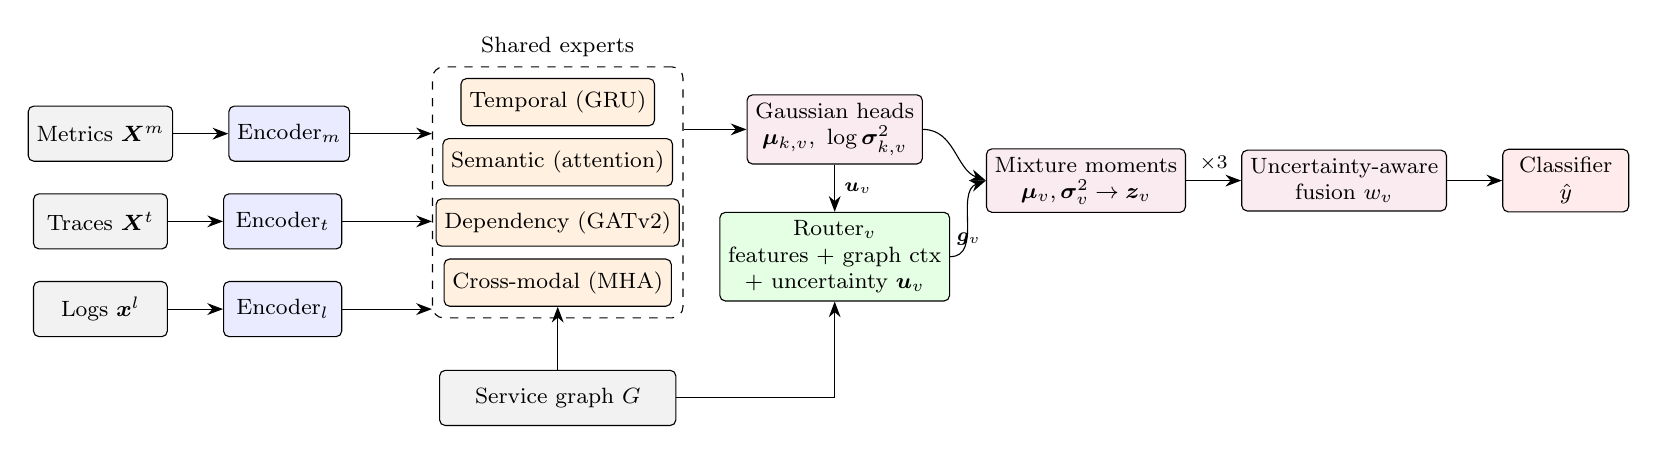
\begin{tikzpicture}[
    font=\footnotesize,
    >={Stealth[length=2mm]},
    box/.style={draw, rounded corners=2pt, align=center, minimum height=7mm, inner sep=3pt},
    inp/.style={box, fill=gray!10, minimum width=17mm},
    enc/.style={box, fill=blue!8, minimum width=15mm},
    exp/.style={box, fill=orange!12, minimum width=22mm, minimum height=6mm},
    rt/.style={box, fill=green!10, minimum width=22mm},
    op/.style={box, fill=purple!8, minimum width=22mm},
    node distance=4mm and 7mm]
  % inputs and encoders
  \node[inp] (xm) {Metrics $\bm{X}^m$};
  \node[inp, below=of xm] (xt) {Traces $\bm{X}^t$};
  \node[inp, below=of xt] (xl) {Logs $\bm{x}^l$};
  \node[enc, right=of xm] (em) {Encoder$_m$};
  \node[enc, right=of xt] (et) {Encoder$_t$};
  \node[enc, right=of xl] (el) {Encoder$_l$};
  \draw[->] (xm) -- (em); \draw[->] (xt) -- (et); \draw[->] (xl) -- (el);
  % shared experts
  \node[exp, right=14mm of em, yshift=4mm] (e1) {Temporal (GRU)};
  \node[exp, below=1.5mm of e1] (e2) {Semantic (attention)};
  \node[exp, below=1.5mm of e2] (e3) {Dependency (GATv2)};
  \node[exp, below=1.5mm of e3] (e4) {Cross-modal (MHA)};
  \begin{scope}[on background layer]
    \node[draw, dashed, rounded corners, fit=(e1)(e4), inner sep=4pt, label={[font=\footnotesize]above:Shared experts}] (experts) {};
  \end{scope}
  \draw[->] (em.east) -- (experts.west |- em.east);
  \draw[->] (et.east) -- (experts.west |- et.east);
  \draw[->] (el.east) -- (experts.west |- el.east);
  % heads
  \node[op, right=8mm of experts, yshift=8mm] (heads) {Gaussian heads\\$\bm{\mu}_{k,v},\ \log\bm{\sigma}^2_{k,v}$};
  \node[rt, below=6mm of heads] (router) {Router$_v$\\features + graph ctx\\+ uncertainty $\bm{u}_v$};
  \draw[->] (experts.east |- heads.west) -- (heads.west);
  \draw[->] (heads.south) -- node[right, font=\scriptsize]{$\bm{u}_v$} (router.north);
  % mixture, fusion, classifier
  \node[op, right=8mm of heads, yshift=-6.5mm] (mix) {Mixture moments\\$\bm{\mu}_v,\bm{\sigma}^2_v\rightarrow\bm{z}_v$};
  \draw[->] (heads.east) to[out=0, in=160] (mix.west);
  \draw[->] (router.east) to[out=0, in=200] node[below, font=\scriptsize]{$\bm{g}_v$} (mix.west);
  \node[op, right=7mm of mix] (fus) {Uncertainty-aware\\fusion $w_v$};
  \node[box, fill=red!8, right=7mm of fus, minimum width=16mm] (cls) {Classifier\\$\hat{y}$};
  \draw[->] (mix) -- node[above, font=\scriptsize]{$\times3$} (fus);
  \draw[->] (fus) -- (cls);
  % graph
  \node[inp, below=8mm of e4, minimum width=30mm] (g) {Service graph $G$};
  \draw[->] (g.north) -- (e4.south);
  \draw[->] (g.east) -| (router.south);
\end{tikzpicture}}
\caption{Architecture of \ugmoe. The experts are shared by the three modalities; the router, the
Gaussian mixture and the fusion input are computed per modality $v$. A learned modality embedding tells the
shared experts which modality they are processing.}
\label{fig:arch}
\end{figure*}

\subsection{Modality Encoders}
\label{sec:enc}
Each modality is projected per service and per time step into a $D$-dimensional space, and a learned
modality embedding $\bm{e}_v$ is added:
\begin{equation}
  \bm{H}^{v}_{i,\tau} = \bm{W}_v \bm{X}^{v}_{i,\tau} + \bm{b}_v + \bm{e}_v ,\qquad \tau=1,\dots,T_v .
\end{equation}
Logs have no time axis ($T_l=1$). The node vector $\bm{h}^v_i=\frac{1}{T_v}\sum_\tau\bm{H}^v_{i,\tau}$
summarises service $i$ in modality $v$.

\subsection{Shared Experts}
\label{sec:experts}
Four experts capture different structure in the data. They are shared by all modalities, so one expert
learns, for example, temporal dynamics from both metrics and traces.
\begin{itemize}
  \item \textbf{Temporal expert:} a GRU~\cite{cho2014gru} over $\bm{H}^v_{i,1:T}$ for each service; its last hidden
  state captures trends and bursts.
  \item \textbf{Semantic expert:} a pre-norm Transformer encoder layer~\cite{vaswani2017attention}
  (4 heads) over the $N$ service vectors. It relates services by content, independently of the graph.
  \item \textbf{Dependency expert:} a GATv2 layer~\cite{brody2022gatv2} (4 heads, residual connection) over
  the service graph $G$, followed by ELU and layer normalisation. It propagates evidence along call edges.
  \item \textbf{Cross-modal expert:} multi-head attention in which a service's vector in modality $v$
  queries the same service's vectors in all three modalities, with a residual connection and layer
  normalisation. It lets a sparse modality borrow evidence from the others.
\end{itemize}
Each expert returns one vector per service, which is pooled over services with
$\operatorname{pool}(\bm{h}_{1:N})=\bm{W}_p[\operatorname{mean}_i\bm{h}_i;\max_i\bm{h}_i]$, giving
$\bm{o}_{k,v}\in\mathbb{R}^D$.

\subsection{Probabilistic Expert Heads}
\label{sec:prob}
Two linear heads per expert map $\bm{o}_{k,v}$ to a mean and a log-variance,
\begin{equation}
  \bm{\mu}_{k,v}=\bm{W}^{\mu}_k\bm{o}_{k,v},\qquad
  \bm{s}_{k,v}=\operatorname{clip}\!\left(\bm{W}^{s}_k\bm{o}_{k,v},-8,8\right),\qquad
  \bm{\sigma}^2_{k,v}=e^{\bm{s}_{k,v}} .
\end{equation}
Predicting the \emph{log}-variance keeps the variance positive and the optimisation well conditioned.
Because every expert predicts its own uncertainty \emph{before} routing, the router can use it. This
resolves the circularity of computing a single uncertainty from the routed mixture and then feeding it
back to the router.

\subsection{Graph- and Uncertainty-Guided Routing}
\label{sec:router}
For modality $v$, the router input concatenates three parts: the pooled modality features, a graph
context vector from a graph convolution~\cite{kipf2017gcn} over the node vectors, and the expected
log-variance of each expert:
\begin{align}
  \bm{c}_v &= \operatorname{pool}\!\big(\operatorname{ELU}(\operatorname{GraphConv}_G(\bm{h}^v_{1:N}))\big), \\
  u_{v,k} &= \tfrac{1}{D}\textstyle\sum_{d} s_{k,v,d}, \\
  \bm{g}_v &= \operatorname{softmax}\!\Big(\operatorname{MLP}_v\big([\operatorname{pool}(\bm{h}^v_{1:N});\,\bm{c}_v;\,\bm{u}_v]\big)/\tau\Big),
\end{align}
where $\tau$ is a temperature. Each modality has its own router, because the same expert can be reliable
for metrics and unreliable for logs. Routing is soft and dense, since $K=4$ makes sparsity unnecessary.

\subsection{Mixture Moments and Sampling}
\label{sec:moments}
The routed experts define a Gaussian mixture. We summarise it by its first two moments,
\begin{align}
  \bm{\mu}_v &= \textstyle\sum_k g_{v,k}\,\bm{\mu}_{k,v}, \\
  \bm{\sigma}^2_v &= \textstyle\sum_k g_{v,k}\big(\bm{\sigma}^2_{k,v}+\bm{\mu}_{k,v}^{2}\big)-\bm{\mu}_v^{2},
\end{align}
with $\bm{\sigma}^2_v$ floored at $10^{-6}$. The total variance includes the disagreement between experts
as well as their individual variances. During training we sample
$\bm{z}_v=\bm{\mu}_v+\bm{\sigma}_v\odot\bm{\epsilon}$, $\bm{\epsilon}\sim\mathcal{N}(\bm{0},\bm{I})$~\cite{kingma2014vae};
at evaluation we use $\bm{z}_v=\bm{\mu}_v$, so predictions are deterministic.

\subsection{Uncertainty-Aware Fusion and Classification}
\label{sec:fusion}
A shared scoring network rates each modality from its mean and its average log-variance, and a softmax over
the three modalities gives the fusion weights:
\begin{align}
  w_v &= \frac{\exp\big(\phi([\bm{\mu}_v;\ \overline{\log\bm{\sigma}^2_v}])\big)}{\sum_{v'}\exp\big(\phi([\bm{\mu}_{v'};\ \overline{\log\bm{\sigma}^2_{v'}}])\big)}, \\
  \bm{z} &= \textstyle\sum_v w_v\,\bm{z}_v ,\qquad \hat{\bm{p}}=\operatorname{softmax}(\operatorname{MLP}(\bm{z})).
\end{align}
The scoring network $\phi$ can learn to give a modality less weight when its predicted uncertainty is high.

\subsection{Training Objective}
The loss is the cross-entropy plus a KL regulariser towards a standard normal prior, averaged over the
modalities:
\begin{equation}
  \mathcal{L}=\mathrm{CE}(\hat{\bm{p}},y)+\lambda_{\mathrm{KL}}\,\frac{1}{3}\sum_v
  \frac{1}{2}\,\overline{\big(\bm{\mu}_v^2+\bm{\sigma}^2_v-1-\log\bm{\sigma}^2_v\big)} .
  \label{eq:loss}
\end{equation}
The bar denotes the mean over dimensions and the batch. A load-balancing term is implemented but disabled
by default, because the dense router did not collapse.

\begin{algorithm}[!t]
\caption{Forward pass of \ugmoe{} for one batch}
\label{alg:forward}
\begin{algorithmic}[1]
\Require graph $G$; observations $\bm{X}^m,\bm{X}^t,\bm{x}^l$; training flag
\For{$v \in \{m, t, l\}$}
  \State $\bm{H}^v \gets \mathrm{Enc}_v(\bm{X}^v)+\bm{e}_v$; \ $\bm{h}^v_i\gets\operatorname{mean}_\tau \bm{H}^v_{i,\tau}$
  \For{$k = 1,\dots,K$}
    \State $\bm{o}_{k,v} \gets \operatorname{pool}(\mathrm{Expert}_k(\bm{H}^v,\bm{h}^v,G,\bm{h}^{m,t,l}))$
    \State $\bm{\mu}_{k,v}, \bm{s}_{k,v} \gets$ heads$_k(\bm{o}_{k,v})$; \ $u_{v,k}\gets\operatorname{mean}_d\bm{s}_{k,v}$
  \EndFor
  \State $\bm{g}_v \gets \operatorname{softmax}(\mathrm{Router}_v(\operatorname{pool}\bm{h}^v, \bm{c}_v(G), \bm{u}_v)/\tau)$
  \State $\bm{\mu}_v,\bm{\sigma}^2_v \gets$ mixture moments of $\{(g_{v,k},\bm{\mu}_{k,v},e^{\bm{s}_{k,v}})\}_k$
  \State $\bm{z}_v \gets \bm{\mu}_v+\bm{\sigma}_v\odot\bm{\epsilon}$ \textbf{if} training \textbf{else} $\bm{\mu}_v$
\EndFor
\State $\bm{w}\gets\operatorname{softmax}_v\,\phi([\bm{\mu}_v;\overline{\log\bm{\sigma}^2_v}])$; \ $\bm{z}\gets\sum_v w_v\bm{z}_v$
\State \Return $\hat{\bm{p}}=\operatorname{softmax}(\mathrm{MLP}(\bm{z}))$, loss~\eqref{eq:loss}
\end{algorithmic}
\end{algorithm}

\subsection{Switches, Incremental Construction and Complexity}
Each component has a switch that removes exactly that component:
\begin{itemize}
  \item \emph{graph}: no dependency expert and no graph context in the router;
  \item \emph{MoE}: a single temporal expert and no router;
  \item \emph{dynamic routing}: uniform weights $g_{v,k}=1/K$;
  \item \emph{uncertainty routing}: the router does not see $\bm{u}_v$;
  \item \emph{probabilistic representation}: $\bm{z}_v=\bm{\mu}_v$, no variance and no KL term;
  \item \emph{adaptive fusion}: $w_v=1/3$.
\end{itemize}
Switching the components on in the order plain MoE $\rightarrow$ graph $\rightarrow$ probabilistic
$\rightarrow$ uncertainty routing $\rightarrow$ fusion gives the incremental construction. The first two
steps are our Plain MoE and Graph-MoE baselines, which have exactly the same experts as the full model.
With $D=64$ the full model has 166k parameters on SN (167k on TT), against 242k for MUAD and 303k for the GAT
baseline.

% =============================================================================
\section{Pitfalls in the Existing Evaluation Protocol}
\label{sec:pitfalls}

We examined the MUAD paper~\cite{dou2026muad}, its public implementation and the processed SN data it
ships. The data match the paper's description: 15 log templates, and 3,366 training and 2,244 test windows,
an exact 60/40 split.

\subsection{Leakage through Overlapping Windows}
The paper states that 60\% of the samples are selected at random for training, with windows of length 10
and stride 1. Window $t$ covers seconds $t,\dots,t+9$ and window $t+1$ covers $t+1,\dots,t+10$. The first nine
metric steps of window $t+1$ equal the last nine of window $t$, so the shipped windows can be chained back
into their four original fault-injection runs (1,402 / 1,402 / 1,404 / 1,402 windows; every window is
covered and no chaining is ambiguous). After this reconstruction, \textbf{1,882 of the 2,244 test windows
(83.9\%) have a training window as their immediate one-second-shifted neighbour}. Most test windows are thus
near-copies of training data.

\subsection{Imbalance and the Trivial Predictor}
In the shipped data, 83\% of the test windows are anomalous. A constant ``anomalous'' predictor therefore
reaches precision 0.829, recall 1.0 and F1 0.906 without looking at the input. The ``only log'' variant in
MUAD's own ablation reports exactly these values (F1 0.9064, recall 1.000, precision 0.8289), which suggests
that it learned this constant predictor. Anomaly-class F1 alone therefore says little on this data, and we
report macro-F1 and a trivial row throughout.

\subsection{Implementation Defects}
The reference implementation has four further defects:
\begin{enumerate}
  \item \emph{Test-set model selection.} The training loop evaluates on the test set and keeps the epoch with
  the highest test F1. Early stopping monitors the training loss, so no held-out signal is used.
  \item \emph{Stochastic evaluation.} The reparameterisation is applied in evaluation mode as well, so
  repeated evaluations of the same checkpoint differ (0.9884 vs 0.9882 F1 in our runs).
  \item \emph{Incorrect KL term.} The encoder outputs a variance $\sigma^2\in(0,1)$ through a sigmoid, but the
  regulariser is $-\tfrac12\sum(1+\sigma^2-\mu^2-e^{\sigma^2})$, i.e.\ the variance is used where the
  log-variance belongs. With $f(s)=1+s-e^{s}$ we have $f(0)=0$ and $f'(s)<0$ for $s>0$, so this term is
  minimised at $\sigma^2=0$. It drives the variance to zero instead of towards the unit-variance prior.
  \item \emph{Invisible log features.} The shipped log features lie in $[0,\,6.06\times10^{-10}]$ and are not
  normalised. Removing logs or traces from the test inputs of a trained MUAD checkpoint leaves its
  predictions unchanged (F1 0.9884 in all three cases), while removing metrics reduces it to the trivial
  predictor. On this data MUAD is effectively a metrics-only detector.
\end{enumerate}

\subsection{How Much of the Score Is Protocol?}
Table~\ref{tab:protocol} evaluates MUAD under progressively stricter protocols. With validation-based
selection but the paper's random split, we reproduce the paper's number to within 0.5 points (0.988 vs
0.993), which validates our reproduction. A leak-free split of the same data lowers macro-F1 from 0.965 to
0.932. On SN rebuilt from the raw recordings, which includes fault-free runs and a later, unseen fault run,
MUAD reaches 0.908 F1 and 0.925 macro-F1 over five seeds. With the paper's own hyperparameters (learning rate
$10^{-3}$, 120 epochs) it scores lower on that data (0.793 vs 0.922 macro-F1, seed 42), so the shared settings
we use favour MUAD.

\begin{table}[!t]
\caption{MUAD on SN under progressively stricter protocols.}
\label{tab:protocol}
\centering
\footnotesize
\setlength{\tabcolsep}{4pt}
\begin{tabular}{@{}llccc@{}}
\toprule
Data & Split / selection & F1 & Macro-F1 & Trivial F1 \\
\midrule
MUAD paper, Dataset C & random, test-selected & 0.993 & -- & -- \\
Shipped SN windows & random, val-selected & 0.988 & 0.965 & 0.906 \\
Shipped SN windows & run-level, val-selected & 0.977 & 0.932 & 0.908 \\
SN rebuilt (5 seeds) & run-level, val-selected & 0.908 & 0.925 & 0.579 \\
\bottomrule
\end{tabular}
\end{table}

% =============================================================================
\section{Experimental Setup}
\label{sec:setup}

\subsection{Datasets}
We use the SocialNetwork (SN, from DeathStarBench~\cite{gan2019deathstarbench}) and TrainTicket
(TT~\cite{zhou2018trainticket}) recordings published with Eadro~\cite{lee2023eadro}. We rebuild both from the
raw files with our own pipeline, which does the following:
\begin{itemize}
  \item verifies archive checksums;
  \item detects per-run clock offsets between spans, logs and metrics (SN spans are offset by $+8$~h);
  \item builds 10-s windows on a 1-s grid, with stride 1 on SN and 5 on TT;
  \item labels a window anomalous if it overlaps an injected fault by at least 1~s.
\end{itemize}
The features are:
\begin{itemize}
  \item \emph{metrics}: 7 raw container metrics per service per second;
  \item \emph{traces}: $\log(1+\cdot)$ of the mean span latency per service per second;
  \item \emph{logs}: $\log(1+\cdot)$ counts of Drain~\cite{he2017drain} templates (at most the 30 most frequent
  plus an ``other'' bucket), mined after masking numbers, addresses and identifiers.
\end{itemize}
Unlike the shipped MUAD data, both datasets include fault-free runs. The faults are CPU load, network delay and
network loss. Table~\ref{tab:data} summarises the data. TT spans cover only 2--4\% of seconds, so TT is in
practice a metrics-and-logs dataset, and its windows are dominated by anomalies.

\begin{table}[!t]
\caption{Datasets rebuilt from the raw Eadro recordings.}
\label{tab:data}
\centering
\footnotesize
\setlength{\tabcolsep}{3.5pt}
\begin{tabular}{@{}lcc@{}}
\toprule
 & SN & TT \\
\midrule
Services / dependency edges & 12 / 24 & 27 / 44 \\
Fault runs / fault-free runs & 4 / 3 & 9 / 2 \\
Window length / stride & 10\,s / 1\,s & 10\,s / 5\,s \\
Windows (train / val / test) & 4,236 / $\approx$2,835 / $\approx$2,835 & 8,397 / 3,228 / 3,226 \\
Anomalous share of test & 40.7\% & 67.9\% \\
Trivial test F1 / macro-F1 & 0.579 / 0.289 & 0.809 / 0.404 \\
Trace coverage (seconds with spans) & 58--95\% & 2--4\% \\
\bottomrule
\end{tabular}
\end{table}

\subsection{Leak-Free Protocol}
All models share one protocol:
\begin{itemize}
  \item \emph{Run-level chronological split.} Fault runs are ordered in time; the last 20\% form the test set,
  the 20\% before them the validation set, and the rest the training set. On SN, the three fault-free runs are
  assigned whole, one to each split. TT has only two fault-free runs, so each is cut chronologically into
  60/20/20\% segments; windows straddling a cut are dropped. No window crosses splits, and every split
  contains normal operation.
  \item \emph{Normalisation.} Per-channel z-scores for every modality, with statistics computed on the
  training split only.
  \item \emph{Model selection.} The checkpoint with the best \emph{validation} macro-F1 (ties broken by PR-AUC)
  is restored, and the test set is evaluated exactly once. We select on macro-F1 rather than anomaly-F1,
  because the constant predictor can win the latter on anomaly-heavy validation sets.
  \item \emph{Seeds.} Five seeds (42, 123, 456, 789, 999). Training is deterministic for a given seed, and
  significance is assessed with a paired $t$-test over seeds.
\end{itemize}

\subsection{Baselines}
\begin{itemize}
  \item \textbf{MUAD}~\cite{dou2026muad}, the published implementation trained on its own objective
  (cross-entropy, confidence loss and KL) and evaluated with our protocol. Its test-time sampling is left
  as published; it changes F1 by less than $10^{-3}$.
  \item \textbf{GAT}~\cite{velickovic2018gat}: two GATv2 layers~\cite{brody2022gatv2} over the service graph, with node features that
  concatenate the time-averaged metric, trace and log embeddings, followed by mean pooling and an MLP. It
  represents graph-based multimodal detectors in the style of Eadro.
  \item \textbf{Plain MoE} and \textbf{Graph-MoE}: the first two steps of the incremental construction, i.e.\
  \ugmoe{} without the uncertainty components and without (or with) the graph.
  \item \textbf{Trivial}: always predicts ``anomalous''.
\end{itemize}

\subsection{Metrics}
We report precision, recall and F1 of the anomalous class, F1 of the normal class, \textbf{macro-F1} (the
primary metric), PR-AUC and ROC-AUC. We also report recall per fault type and the false-positive rate on
normal windows.

\subsection{Implementation Details}
All models are implemented in PyTorch with DGL~\cite{wang2019dgl} and trained with Adam~\cite{kingma2015adam}
under identical settings: learning rate $5\times10^{-4}$, weight decay $10^{-5}$, batch size 50, at most 50
epochs, early stopping with patience 15 on validation, and gradient clipping at norm 0.5. \ugmoe{} uses $D=64$,
4 attention heads, dropout 0.1, $\lambda_{\mathrm{KL}}=0.01$ and $\tau=1$. These defaults were fixed before the
sensitivity study and were not tuned on test data.

% =============================================================================
\section{Results}
\label{sec:results}

We address six research questions.
\begin{itemize}
  \item \textbf{RQ1:} How accurate is \ugmoe{} compared with the baselines?
  \item \textbf{RQ2:} What does each component contribute?
  \item \textbf{RQ3:} What does each modality contribute?
  \item \textbf{RQ4:} How robust is \ugmoe{} to missing and noisy observations?
  \item \textbf{RQ5:} Do routing and uncertainty behave as intended?
  \item \textbf{RQ6:} How sensitive is \ugmoe{} to its hyperparameters?
\end{itemize}
Unless stated otherwise, numbers are test macro-F1, given as mean $\pm$ standard deviation over five seeds.

% -----------------------------------------------------------------------------
\subsection{RQ1: Overall Performance}

\begin{table*}[!t]
\caption{Overall performance (test set, mean $\pm$ std over 5 seeds). $p$: paired $t$-test of macro-F1 against \ugmoe{} (full); bold $p<0.05$.}
\label{tab:main}
\centering
\footnotesize
\setlength{\tabcolsep}{3.2pt}
\begin{tabular}{@{}llcccccccc@{}}
\toprule
& Model & Params & Precision & Recall & F1 & F1 (normal) & \textbf{Macro-F1} & PR-AUC & $p$ \\
\midrule
\multirow{6}{*}{\rotatebox{90}{SN}}
& Trivial (all anomalous) & -- & 0.407 & 1.000 & 0.579 & 0.000 & 0.289 & 0.407 & -- \\
& MUAD~\cite{dou2026muad} & 242k & 0.970\sd{0.014} & 0.853\sd{0.015} & 0.908\sd{0.007} & 0.943\sd{0.004} & 0.925\sd{0.005} & 0.968\sd{0.010} & \pv{0.002} \\
& GAT & 303k & 0.977\sd{0.003} & 0.861\sd{0.078} & 0.914\sd{0.045} & 0.948\sd{0.024} & 0.931\sd{0.035} & 0.989\sd{0.005} & \pv{0.024} \\
& Plain MoE & 115k & 0.991\sd{0.003} & 0.941\sd{0.040} & 0.965\sd{0.021} & 0.977\sd{0.013} & 0.971\sd{0.017} & 0.997\sd{0.001} & 0.948 \\
& Graph-MoE & 144k & 0.989\sd{0.005} & 0.916\sd{0.042} & 0.951\sd{0.022} & 0.969\sd{0.013} & 0.960\sd{0.018} & 0.996\sd{0.001} & 0.241 \\
& \textbf{\ugmoe{} (full)} & 166k & 0.990\sd{0.007} & 0.943\sd{0.027} & \best{0.966}\sd{0.016} & \best{0.978}\sd{0.010} & \best{0.972}\sd{0.013} & 0.996\sd{0.002} & -- \\
\midrule
\multirow{6}{*}{\rotatebox{90}{TT}}
& Trivial (all anomalous) & -- & 0.679 & 1.000 & 0.809 & 0.000 & 0.404 & 0.679 & -- \\
& MUAD~\cite{dou2026muad} & 243k & 0.908\sd{0.014} & 0.504\sd{0.061} & 0.646\sd{0.049} & 0.607\sd{0.015} & 0.626\sd{0.032} & 0.914\sd{0.012} & \pv{0.042} \\
& GAT & 304k & 0.911\sd{0.019} & 0.563\sd{0.084} & 0.692\sd{0.061} & 0.630\sd{0.029} & 0.661\sd{0.044} & 0.925\sd{0.013} & 0.281 \\
& Plain MoE & 116k & 0.911\sd{0.034} & 0.640\sd{0.181} & 0.735\sd{0.092} & 0.661\sd{0.054} & 0.698\sd{0.073} & 0.919\sd{0.020} & 0.724 \\
& Graph-MoE & 145k & 0.938\sd{0.031} & 0.553\sd{0.111} & 0.688\sd{0.088} & 0.645\sd{0.039} & 0.667\sd{0.063} & 0.902\sd{0.045} & 0.446 \\
& \textbf{\ugmoe{} (full)} & 167k & 0.903\sd{0.039} & 0.700\sd{0.215} & \best{0.766}\sd{0.117} & \best{0.681}\sd{0.063} & \best{0.723}\sd{0.090} & 0.917\sd{0.040} & -- \\
\bottomrule
\end{tabular}
\end{table*}

Table~\ref{tab:main} gives the main comparison. \textbf{\ugmoe{} is the best model on both datasets.} On SN
it improves macro-F1 over MUAD by 4.6 points ($p=0.002$) and over GAT by 4.1 points ($p=0.024$). On TT it
improves over MUAD by 9.7 points ($p=0.042$) and over GAT by 6.3 points; the latter difference is not
significant ($p=0.281$) because of the large seed variance on TT. The gains come mainly from recall: on SN,
recall rises from 0.853 (MUAD) to 0.943 at a precision of about 0.99.

\textbf{The full model is statistically tied with the Plain MoE} that uses the same experts (+0.1 on SN,
+2.5 on TT; $p\geq0.72$). Most of the gain over the baselines therefore comes from the shared-expert
mixture rather than from the uncertainty components. On TT, the full model's PR-AUC (0.917) is level with
the baselines' (0.914--0.925). Its higher macro-F1 comes from a better operating point, catching more faults,
rather than from a better ranking of windows.

\begin{table}[!t]
\caption{Recall per fault type and false-positive rate (FPR) on normal windows, clean test set, 5-seed mean.}
\label{tab:types}
\centering
\footnotesize
\setlength{\tabcolsep}{3.5pt}
\begin{tabular}{@{}llcccc@{}}
\toprule
& Model & CPU load & Net.\ delay & Net.\ loss & FPR \\
\midrule
\multirow{2}{*}{SN} & MUAD & 0.658 & \best{0.988} & \best{0.910} & 0.018 \\
                    & \ugmoe{} & \best{0.984} & 0.954 & 0.891 & \best{0.007} \\
\midrule
\multirow{3}{*}{TT} & MUAD & 0.914 & 0.331 & 0.273 & \best{0.109} \\
                    & GAT & 0.876 & 0.461 & 0.353 & 0.119 \\
                    & \ugmoe{} & \best{0.998} & \best{0.594} & \best{0.508} & 0.183 \\
\bottomrule
\end{tabular}
\end{table}

Table~\ref{tab:types} breaks recall down by fault type. On SN, MUAD misses a third of the CPU-load faults,
which accounts for most of the gap; \ugmoe{} detects 98\% of them and also raises fewer false alarms. On TT,
every model detects CPU faults, but network faults are hard: \ugmoe{} detects about twice as many network
delay and loss faults as MUAD, at a higher false-positive rate (18.3\% vs 10.9\%).

% -----------------------------------------------------------------------------
\subsection{RQ2: Component Ablation}

\begin{table}[!t]
\caption{Component ablation: test macro-F1 (5 seeds) and $\Delta$ = ablation $-$ full, with paired $t$-test $p$-values.}
\label{tab:ablation}
\centering
\footnotesize
\setlength{\tabcolsep}{2.6pt}
\begin{tabular}{@{}lcccc@{}}
\toprule
& \multicolumn{2}{c}{SN} & \multicolumn{2}{c}{TT} \\
\cmidrule(lr){2-3}\cmidrule(lr){4-5}
Variant & Macro-F1 & $\Delta$ ($p$) & Macro-F1 & $\Delta$ ($p$) \\
\midrule
\ugmoe{} (full) & 0.972\sd{0.013} & -- & 0.723\sd{0.090} & -- \\
w/o graph & 0.978\sd{0.008} & $+0.6$ (0.21) & 0.741\sd{0.082} & $+1.8$ (0.78) \\
w/o MoE & 0.965\sd{0.028} & $-0.6$ (0.75) & 0.724\sd{0.070} & $+0.1$ (0.97) \\
w/o dynamic routing & 0.977\sd{0.004} & $+0.5$ (0.43) & 0.673\sd{0.030} & $-5.0$ (0.44) \\
w/o uncertainty routing & 0.974\sd{0.015} & $+0.2$ (0.85) & 0.698\sd{0.071} & $-2.6$ (0.65) \\
w/o probabilistic repr. & 0.980\sd{0.008} & $+0.8$ (0.36) & 0.704\sd{0.068} & $-1.9$ (0.44) \\
w/o adaptive fusion & 0.948\sd{0.012} & $\bm{-2.4}$ (0.06) & 0.690\sd{0.132} & $\bm{-3.3}$ (0.68) \\
\bottomrule
\end{tabular}
\end{table}

Table~\ref{tab:ablation} removes one component at a time. \textbf{No single removal changes macro-F1
significantly over five seeds.} Uncertainty-aware adaptive fusion comes closest: it is the only component
whose removal lowers macro-F1 on both datasets ($-2.4$ on SN with $p=0.06$, and $-3.3$ on TT). On TT, removing
dynamic routing ($-5.0$), uncertainty routing ($-2.6$) or the probabilistic representation ($-1.9$) points in
the expected direction, but the differences are well within the seed variance. On SN, which is close to
its ceiling, the graph and probabilistic components make no measurable difference.

Single-seed ablations are misleading on these benchmarks. With seed 42 alone, removing the MoE cost 7.8
points on SN and removing the graph cost 18.8 points on TT; over five seeds these effects become $-0.6$ and
$+1.8$. We therefore report only multi-seed ablations.

% -----------------------------------------------------------------------------
\subsection{RQ3: Modality Contribution}

\begin{table}[!t]
\caption{Modality ablation on SN: \ugmoe{} trained and tested on a subset of modalities (seed 42).}
\label{tab:modality}
\centering
\footnotesize
\begin{tabular}{@{}lc|lc@{}}
\toprule
Modalities & Macro-F1 & Modalities & Macro-F1 \\
\midrule
Metrics & 0.883 & Traces + logs & 0.938 \\
Traces & 0.935 & Metrics + logs & 0.959 \\
Logs & 0.832 & Metrics + traces & 0.929 \\
\midrule
\multicolumn{3}{@{}l}{All three} & \best{0.987} \\
\bottomrule
\end{tabular}
\end{table}

Table~\ref{tab:modality} trains \ugmoe{} on each subset of modalities. After normalisation, every modality
carries substantial signal on its own (0.83--0.94), and traces alone are the strongest. Combining all three
modalities adds 2.8 points over the best pair. This contrasts with the shipped MUAD data, where logs and
traces had no effect (Section~\ref{sec:pitfalls}).

% -----------------------------------------------------------------------------
\subsection{RQ4: Robustness to Missing and Noisy Data}

We perturb the inputs of the trained checkpoints at test time only, using the same random masks and noise
draws for every model:
\begin{itemize}
  \item \emph{D1}: drop one modality entirely;
  \item \emph{D2}: zero each (window, service, modality) observation independently with probability $p$;
  \item \emph{E}: add Gaussian noise with standard deviation equal to a multiple of each channel's training
  standard deviation, on every combination of modalities.
\end{itemize}
Table~\ref{tab:robust} summarises the results, and Fig.~\ref{fig:robust} shows the masking and noise curves.

\begin{table*}[!t]
\caption{Robustness: test macro-F1 under test-time perturbation (5-seed mean). ``Mask $p$'': each observation
zeroed with probability $p$. ``Noise $\sigma$'': Gaussian noise on all modalities, $\sigma$ times the training std.
Trivial macro-F1: SN 0.289, TT 0.404.}
\label{tab:robust}
\centering
\footnotesize
\setlength{\tabcolsep}{4pt}
\begin{tabular}{@{}llcccccccccc@{}}
\toprule
& Model & Clean & $-$metrics & $-$traces & $-$logs & Mask 0.1 & Mask 0.2 & Mask 0.4 & Mask 0.6 & Noise 1 & Noise 2 \\
\midrule
\multirow{4}{*}{SN}
& MUAD & 0.925 & 0.289 & 0.915 & 0.922 & 0.898 & 0.850 & 0.710 & 0.543 & 0.865 & 0.735 \\
& Plain MoE & 0.971 & 0.289 & 0.976 & 0.868 & 0.935 & 0.885 & 0.780 & 0.683 & \best{0.941} & 0.737 \\
& \ugmoe{} w/o probabilistic & \best{0.980} & 0.289 & \best{0.977} & \best{0.975} & \best{0.946} & 0.902 & 0.797 & 0.663 & 0.924 & \best{0.810} \\
& \textbf{\ugmoe{} (full)} & 0.972 & 0.274 & 0.973 & 0.967 & 0.942 & \best{0.903} & \best{0.811} & \best{0.696} & 0.937 & 0.808 \\
\midrule
\multirow{3}{*}{TT}
& MUAD & 0.627 & 0.243 & 0.628 & 0.654 & 0.622 & \best{0.613} & \best{0.568} & \best{0.526} & \best{0.559} & \best{0.537} \\
& GAT & 0.661 & 0.404 & 0.639 & 0.670 & \best{0.636} & 0.605 & 0.529 & 0.452 & \best{0.559} & 0.523 \\
& \textbf{\ugmoe{} (full)} & \best{0.723} & 0.406 & \best{0.711} & \best{0.676} & 0.616 & 0.573 & 0.506 & 0.471 & 0.480 & 0.470 \\
\bottomrule
\end{tabular}
\end{table*}

\begin{figure*}[!t]
\centering
\figorbox{robustness_masking_sn.png}{0.32\textwidth}\hfill
\figorbox{robustness_noise_sn.png}{0.32\textwidth}\hfill
\figorbox{robustness_masking_tt.png}{0.32\textwidth}
\caption{Macro-F1 under random masking (left: SN; right: TT) and under Gaussian noise on all modalities
(middle: SN), 5-seed mean. On SN the gap between \ugmoe{} and MUAD widens as more data is corrupted; on TT
the clean-data lead is lost from 20\% masking on.}
\label{fig:robust}
\end{figure*}

\textbf{On SN, \ugmoe{} stays ahead of MUAD under every perturbation, and the gap grows with the amount of
corruption.} The margin is 4.6 points on clean data and 5.3, 10.1 and 15.3 points at 20\%, 40\% and 60\%
masking; under strong noise ($\sigma=2$) it is 7.3 points. The full model is also ahead of the Plain MoE
under masking (+1.8 at 20\%, +3.1 at 40\%) and strong noise (+7.1), but not consistently across seeds.

\textbf{The probabilistic representation does not explain the robustness.} The model without it is level
with the full model under masking (0.902 vs 0.903 at 20\%, 0.797 vs 0.811 at 40\%) and under noise (0.810 vs
0.808). With seed 42 alone, the ablated model lost 12.8 and 14.9 F1 points at 20\% and 40\% masking; that
checkpoint was an unusually fragile one.

\textbf{All models fail without metrics.} Dropping metrics reduces every model to (or below) the trivial
score on both datasets, whereas dropping traces or logs costs at most 5 points (except the Plain MoE without
logs on SN, $-10.3$). None of the models sees a window without metrics during training, so none learns to
fall back on the other modalities, even though a model \emph{trained} on traces alone reaches 0.935
(Table~\ref{tab:modality}).

\textbf{On TT, the clean-data lead of \ugmoe{} disappears under perturbation.} From 20\% masking on it is below
MUAD and GAT. The seeds behave in two different ways. Two seeds (123, 456) learned a cautious model with low
network-fault recall (0.14--0.36); these collapse to the trivial ``all anomalous'' prediction at only 10\%
masking. The high-recall seeds (42, 789) degrade gradually. On TT, anomaly-F1 is misleading under perturbation:
a collapsing model approaches the trivial anomaly-F1 of 0.809, so its anomaly-F1 \emph{rises}. We therefore
compare macro-F1.

% -----------------------------------------------------------------------------
\subsection{RQ5: Routing and Uncertainty Analysis}

\begin{figure}[!t]
\centering
\figorbox{routing_sn.png}{\columnwidth}
\caption{Routing weights of the metric router per fault type on SN (seed 42). Normal windows are routed
mainly to the dependency expert, CPU-load faults to the cross-modal expert and network faults to the
temporal expert.}
\label{fig:routing}
\end{figure}

We analyse the seed-42 checkpoint of the full model on the test set; Fig.~\ref{fig:routing} shows the
routing weights.

\emph{Experts specialise by fault type.} On SN, the metric router has a normalised entropy of 0.41 (0: one
expert, 1: uniform). It sends normal windows mainly to the dependency expert (0.87) and CPU-load faults to the
cross-modal expert (0.95), and splits network faults with the temporal expert taking about half. On TT,
CPU-load windows also get a dedicated metric expert (the semantic expert, 0.996). Traces are routed mostly to
the cross-modal expert (SN 0.67, TT 0.87), which is consistent with a sparse modality drawing on the others.
On SN, logs are routed almost uniformly (entropy 0.97).

\begin{table}[!t]
\caption{Fusion weights $w_v$ and mean log-variance of the perturbed modality (seed 42, test set).}
\label{tab:fusion}
\centering
\footnotesize
\setlength{\tabcolsep}{3pt}
\begin{tabular}{@{}llccc@{}}
\toprule
& Condition & F1 & $w_m$ / $w_t$ / $w_l$ & $\overline{\log\sigma^2}$ (perturbed) \\
\midrule
\multirow{5}{*}{SN}
& Clean & 0.984 & 0.96 / 0.03 / 0.01 & -- \\
& Noise on metrics, $\sigma=1$ & 0.971 & 0.91 / 0.06 / 0.03 & metric $-0.22\rightarrow-0.07$ \\
& 40\% masking & 0.846 & 0.89 / 0.07 / 0.04 & metric $-0.22\rightarrow+0.09$ \\
& Logs dropped & 0.981 & 0.96 / 0.02 / 0.02 & log $+0.03\rightarrow+0.15$ \\
& Metrics dropped & 0.579 & 0.88 / 0.09 / 0.03 & metric $-0.22\rightarrow-0.02$ \\
\midrule
\multirow{3}{*}{TT}
& Clean & 0.894 & 0.61 / 0.28 / 0.11 & -- \\
& Metrics dropped & 0.809 & 0.13 / 0.79 / 0.09 & metric $-0.28\rightarrow+0.80$ \\
& Noise on logs, $\sigma=1$ & 0.817 & 0.27 / 0.08 / 0.65 & log $-0.03\rightarrow-0.14$ \\
\bottomrule
\end{tabular}
\end{table}

\emph{Uncertainty moves in the right direction, but often by too little.} Table~\ref{tab:fusion} shows that
corrupting a modality raises its predicted log-variance and lowers its fusion weight:
\begin{itemize}
  \item on SN, noise on the metrics lowers their weight from 0.96 to 0.91;
  \item on TT, dropping the metrics raises their log-variance from $-0.28$ to $+0.80$ and moves 79\% of the
  weight to traces.
\end{itemize}
The shift is too small to make the model fall back on other modalities on SN, where metrics keep 88\% of the
weight even when absent. On TT the shift is large, but the fallback modality (traces) is almost empty.

On SN the predicted uncertainty is higher for wrong predictions than for correct ones (mean log-variance
$-0.04$ vs $-0.23$); on TT it does not separate them. We also observe a failure case: noise on the logs makes
the TT model \emph{more} confident in the logs (log-variance $-0.03\rightarrow-0.14$), which raises their weight
from 0.11 to 0.65 and costs 8 F1 points. Learned variance can be overconfident on inputs unlike any seen in
training.

% -----------------------------------------------------------------------------
\subsection{RQ6: Hyperparameter Sensitivity}

\begin{figure}[!t]
\centering
\figorbox{sensitivity_sn.png}{\columnwidth}
\caption{Sensitivity of test macro-F1 on SN to one hyperparameter at a time (seed 42; the default is
marked).}
\label{fig:sens}
\end{figure}

\begin{table}[!t]
\caption{One-at-a-time sensitivity on SN (seed 42; default value in bold, default macro-F1 0.987).}
\label{tab:sens}
\centering
\footnotesize
\setlength{\tabcolsep}{3pt}
\begin{tabular}{@{}ll@{}}
\toprule
Parameter & Value $\rightarrow$ macro-F1 \\
\midrule
Experts $K$ & 1: 0.909 \quad 2: 0.988 \quad 3: 0.984 \quad \textbf{4}: 0.987 \\
Hidden size $D$ & 16: 0.980 \quad 32: 0.978 \quad \textbf{64}: 0.987 \quad 128: 0.973 \\
$\lambda_{\mathrm{KL}}$ & 0.001: 0.979 \quad \textbf{0.01}: 0.987 \quad 0.1: 0.953 \quad 1: 0.972 \\
Temperature $\tau$ & 0.5: 0.969 \quad \textbf{1}: 0.987 \quad 2: 0.983 \\
Learning rate & $10^{-4}$: 0.982 \quad $\bm{5\cdot10^{-4}}$: 0.987 \quad $10^{-3}$: 0.985 \\
Window length & 5\,s: 0.956 \quad \textbf{10\,s}: 0.987 \quad 20\,s: 0.973 \\
\bottomrule
\end{tabular}
\end{table}

Table~\ref{tab:sens} and Fig.~\ref{fig:sens} vary one hyperparameter at a time. The defaults are the best
setting, or within 0.2 points of it, for every parameter. Only a single expert ($-7.8$) and a large KL weight
($\lambda_{\mathrm{KL}}=0.1$, $-3.4$) hurt clearly; the other differences are within single-seed noise. A model
four times wider ($D=128$) is not better, so the results are not driven by capacity.

% =============================================================================
\section{Discussion}
\label{sec:discussion}

\subsection{What the Evidence Supports}
On a leak-free protocol and over five seeds, \ugmoe{} detects anomalies significantly better than the
uncertainty-aware baseline MUAD on two benchmarks, and better than a graph attention baseline on SN, with
fewer parameters. It catches fault types that the baselines miss (CPU faults on SN, network faults on TT).
On SN it degrades more slowly than MUAD as observations go missing.

\subsection{What It Does Not Support}
We could not attribute these gains to individual components. A plain mixture of the same shared experts
is statistically tied with the full model; no single ablation is significant at five seeds; and the
robustness on SN is not explained by the probabilistic representation. Adaptive fusion is the most useful
component, but its effect is not significant either. On TT, \ugmoe{} is less robust than the baselines under
perturbation, and its seed variance is high. These findings matter for the field: several effects that a
single seed made look large (the MoE on SN, the graph on TT, the probabilistic representation under masking)
disappeared with five seeds. Claims about components of multimodal detectors should therefore rest on
multi-seed experiments with significance tests.

\subsection{Lessons on Evaluation}
Three practices changed the conclusions of this study and should be standard.
\begin{enumerate}
  \item Split by run, chronologically, and never at random across overlapping windows.
  \item Include fault-free operation in every split, and report macro-F1 together with a trivial-predictor
  row, because anomaly-class F1 rewards predicting ``anomalous'' everywhere.
  \item Select checkpoints on a validation set, using a metric that the trivial predictor cannot win.
\end{enumerate}
With these practices, MUAD's F1 on SN falls from 0.993 to 0.908, while the ranking among the stronger models
becomes informative.

\subsection{Threats to Validity}
\emph{Internal.} All models share one implementation of the data pipeline, split, normalisation, selection
and metrics, which removes protocol differences but could hide an error common to all of them. We
mitigated this with per-run alignment diagnostics, by reproducing MUAD's published number under its own
protocol, and with deterministic training per seed. MUAD is evaluated with our shared hyperparameters; its
paper's own settings performed worse on our data.

\emph{Split.} On TT, the fault-free test segments come from the same two runs as the fault-free training
segments (with no shared seconds). There is no time gap at the cuts, and the log templates are mined over
all runs (an unsupervised, label-free step).

\emph{External.} Both benchmarks are small: the SN test set contains one fault run and one fault-free run, and
TT traces are nearly empty, so TT cannot test trace-based fallback. The results may not transfer to
production systems with different fault types, scale or telemetry.

\emph{Statistical.} Five seeds give paired tests limited power. Non-significant differences, including those
of the ablations, are inconclusive rather than evidence of no effect. The routing, uncertainty and
sensitivity analyses use a single seed.

\subsection{Limitations and Future Work}
No model degrades gracefully when metrics are missing. Training with modality dropout, i.e.\ randomly
removing whole modalities during training, is the natural remedy and is left for future work. Learned
variance is overconfident on unfamiliar noise, which calls for calibration or distribution-shift-aware
uncertainty. On TT, \ugmoe{} trades a higher false-positive rate for recall; a threshold chosen on validation
data would make this trade-off explicit. Extending the model to root-cause localisation is a further
direction.

% =============================================================================
\section{Conclusion}
\label{sec:conclusion}
We showed that near-perfect scores reported for multimodal anomaly detection on the SN benchmark arise
largely from leakage between overlapping windows, class imbalance and test-set model selection. We proposed
a leak-free protocol and \ugmoe, a mixture of shared specialised experts with graph- and uncertainty-guided
routing and uncertainty-aware fusion. Under this protocol and over five seeds, \ugmoe{} outperforms MUAD by
4.6 macro-F1 points on SN and 9.7 points on TT, with 31\% fewer parameters, and degrades more slowly than MUAD
when observations go missing on SN. The contribution of its individual uncertainty components could not be
established at this scale. We hope that the protocol, together with this candid accounting of both positive and
negative results, makes future comparisons in this area more reliable.

% =============================================================================
\section*{Data and Code Availability}
The datasets are the public Eadro recordings~\cite{lee2023eadro}. The preprocessing pipeline, model, training
protocol, per-seed checkpoints and the script that regenerates every table and figure of this paper will be
released upon publication.

\bibliographystyle{IEEEtran}
\bibliography{references}

\end{document}
